\documentclass[]{beamer}
\usepackage{beamerthemesplit}
\usepackage{graphics,epsfig}
\usepackage{pstricks}
\usepackage{graphicx}
\usepackage{hyperref}
\usepackage{subfigure}
\usepackage{listings}
\usepackage{courier}
\usepackage{multirow}
\usepackage{xspace}
\usepackage{tikz}


\mode<presentation>
{ \usetheme{Boadilla}
  \setbeamercovered{transparent}
  \setbeamertemplate{items}[circle]
  \setbeamertemplate{theorems}[numbered]
  \setbeamertemplate{footline}[frame number]
  \setbeamercolor{frametitle}{fg=black,bg=white!900}
}
 
%\useinnertheme[shadow=true]{rounded}
\useoutertheme{shadow}
\usecolortheme{whale}

\newcommand\blfootnote[1]{
  \begingroup
  \renewcommand\thefootnote{}\footnote{#1}
  \addtocounter{footnote}{-1}
  \endgroup
}

\mode
<all>

\title{C Programming}
\author{Wan-Lei Zhao}

\makeatletter
\DeclareRobustCommand\onedot{\futurelet\@let@token\@onedot}

\makeatother

\begin{document}
\begin{frame}
   \begin{center}
    \vspace{24pt}
    \Huge\textbf{C Programming}\blfootnote{Email: wlzhao@xmu.edu.cn, copyrights are fully reserved by the author.}\\
     \Huge{Lecture 5: Functions and MACROs}
    \begin{figure}
    	\begin{center}
    		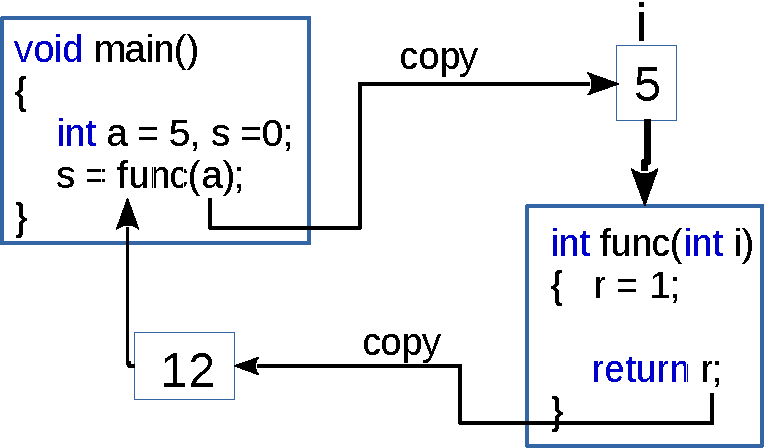
\includegraphics[width=0.32\linewidth]{figs/arg2para0.pdf}
    	\end{center}
    \end{figure}
  \end{center}
  \begin{align*}
   \vspace{18pt}
      \large{\mbox{Lecturer:}~Dr.~\mbox{Wan-Lei~~Zhao}} \\
      \large{Spring~~Semester~~2022} \\
   \vspace{30pt}
  \end{align*}
\end{frame}

\definecolor{cornblue}{HTML}{6495ED}
\definecolor{navyblue}{HTML}{000080}
\definecolor{midnblue}{HTML}{191970}
\definecolor{lghtblue}{HTML}{B0C4DE}
\setbeamercolor{background}{fg=black, bg=lghtblue}
\setbeamercolor{palette primary}{fg=white, bg=lghtblue}
\setbeamercolor{palette secondary}{fg=black, bg=cornblue}
\setbeamercolor{palette tertiary}{fg=black, bg=lghtblue}
\setbeamercolor{palette quaternary}{fg=black, bg=lghtblue}
\setbeamercolor{frametitle}{fg=black, bg=white}
\definecolor{ballblue}{rgb}{0.13, 0.67, 0.8}
\definecolor{cornflowerblue}{rgb}{0.39,0.58,0.93}
\definecolor{babyblueeyes}{rgb}{0.63, 0.79, 0.95}

\setbeamertemplate{footline}
{
  \leavevmode%
  \hbox{%
  \begin{beamercolorbox}[wd=.275\paperwidth,ht=2.25ex,dp=1ex,center]{author in head/foot}%
    \usebeamerfont{author in head/foot}\insertshortauthor
  \end{beamercolorbox}%
  \begin{beamercolorbox}[wd=.44\paperwidth,ht=2.25ex,dp=1ex,center]{title in head/foot}%
    \usebeamerfont{title in head/foot}\insertshorttitle\hspace*{3em}
    \hspace*{1ex}
  \end{beamercolorbox}%
  \begin{beamercolorbox}[wd=.285\paperwidth,ht=2.25ex,dp=1ex,center]{date/foot}%
    \usebeamerfont{title in head/foot}\hspace*{2em}
    \insertframenumber{} / \inserttotalframenumber\hspace*{1ex}
  \end{beamercolorbox}}%
  \vskip0pt
}



% preset-listing options
\lstset{
  backgroundcolor=\color{white},   
  basicstyle=\footnotesize,    
  language=c,
  breakatwhitespace=false,         
  breaklines=true,                 % sets automatic line breaking
  captionpos=b,                    % sets the caption-position to bottom
  commentstyle=\color{ballblue},    % comment style
  extendedchars=true,              
  frame=single,                    % adds a frame around the code     
  keywordstyle=\color{blue},       % keyword style
  numbers=left,                    
  numbersep=5pt,                   
  numberstyle=\tiny\color{blue}, 
  rulecolor=\color{babyblueeyes},
  stepnumber=1,              
  stringstyle=\color{black},     % string literal style
  tabsize=4,                       % sets default tabsize to 4 spaces
  title=\lstname                   
}


\section{Functions: declaration, definition and calling}
\label{sec:func}
\begin{frame}<beamer>
    \frametitle{Outline}
    \tableofcontents[currentsection]
\end{frame}

\begin{frame}[fragile]{Overview}

\begin{columns}
\begin{column}{0.45\linewidth}
\begin{itemize}
	\item {Functions we know}
\end{itemize}
\begin{lstlisting}
int main(.);
int printf(..);
int scanf(.);
float sqrt(.);
float floor(.);
float fabs(.); 
\end{lstlisting}
\end{column}
\begin{column}{0.45\linewidth}
\begin{itemize}
	\item {Functions in math}
\end{itemize}
\begin{eqnarray}
f(x)=sin(x) \nonumber\\
g(x)=x^2 \nonumber
\end{eqnarray}
\end{column}
\end{columns}
\begin{itemize}
	\item {They are actually comparable}
	\item {Function in C is more general}
	\item {We are going to learn to organize our codes into functions (blocks)}
\end{itemize}
\end{frame}

\begin{frame}[fragile]{Advantages of function (1)}
\begin{itemize}
	\item {We are already familiar with functions}
\end{itemize}
\begin{lstlisting}
int main(.); //entrance of the program
int printf(..); //print things onto screen
int scanf(.);  //read input from keyboard
float sqrt(.); //take square root
float floor(.); //take maximum number smaller than input
float fabs(.); //take absolute value of a float number
\end{lstlisting}
\begin{itemize}
	\item {Advantages}
	\begin{itemize}
		\item {No need to repeat others work (reinvent the wheel)}
		\item {No need to write things again and again}
		\item {Your codes become cleaner}
	\end{itemize}
\end{itemize}
\end{frame}

\begin{frame}[fragile]{Introdution of function (1)}
\begin{itemize}
	\item {Let's start with a simple example}
\end{itemize}
\begin{lstlisting}
#include <stdio.h>
void hi(int i) //<---declaration of function "hi"
{
   printf("Hello %d\n", i);
}

int main()
{
   int i = 0;
   for(i = 0; i < 5; i++)
      hi(i); //<-- call function hi(int i)
   return 0; //return value to the one who calls it
}
\end{lstlisting}
\vspace{-0.15in}
\begin{itemize}
	\item {We call \textbf{hi}() inside main}
	\item {``\textbf{main}()'' cannot be called by any other function}
\end{itemize}
\end{frame}

\begin{frame}[fragile]{Declaration of function (1)}
\begin{itemize}
	\item {Declare a function for $n!$}
\end{itemize}
\begin{lstlisting}
long fact(int i); //<-- this is the declaration

int main()
{
   int i = 5, f = 0;
   f = fact(i);
   return 0; //return value to the one who calls it
}
\end{lstlisting}
\vspace{-0.15in}
\begin{itemize}
	\item {The name should be \textbf{unique}}
	\item {There is should be input parameter(s) along with the types}
	\item {There is should be output value type}
\end{itemize}
\end{frame}


\begin{frame}[fragile]{Declaration of function (2)}
\begin{itemize}
	\item {Declare a function for $n!$}
\end{itemize}
\begin{figure}
	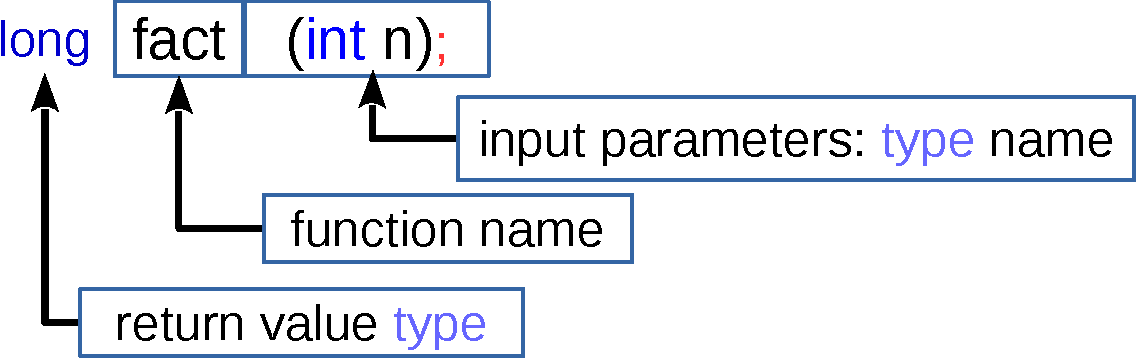
\includegraphics[width=0.8\linewidth]{figs/func_declar.pdf}
\end{figure}
\vspace{-0.15in}
\begin{itemize}
	\item {The name should be \textbf{unique}}
	\item {There should be input parameter(s) along with the types}
	\item {There should be output value type}
	\item {If there is nothing, the returning type is \textcolor{blue}{int}}
\end{itemize}
\end{frame}

\begin{frame}[fragile]{Declaration of function (3)}
\begin{itemize}
	\item {Declare a function for $n!$}
\end{itemize}
\begin{figure}
	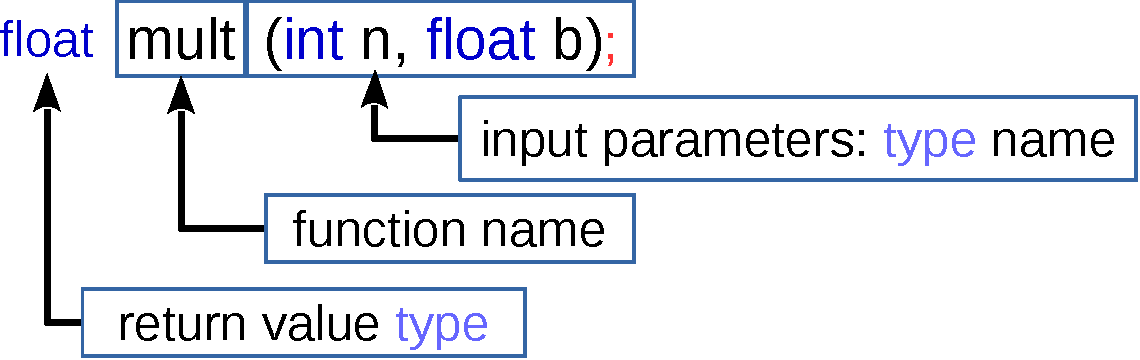
\includegraphics[width=0.8\linewidth]{figs/func_declar2.pdf}
\end{figure}
\vspace{-0.15in}
\begin{itemize}
	\item {The name should be \textbf{unique}}
	\item {There should be input parameter(s) along with the types}
	\item {There should be output value type}
	\item {If there is nothing, the returning type is \textcolor{blue}{int} by default}
\end{itemize}
\end{frame}

\begin{frame}[fragile]{Define a function (1)}
\begin{itemize}
	\item {Declare a function for $n!$}
\end{itemize}
\begin{lstlisting}
long fact(int i); //<-- this is the declaration

int main()
{
   int i = 5, f = 0;
   f = fact(i);
   return 0; //return value to the one who calls it
}
\end{lstlisting}
\vspace{-0.15in}
\begin{center}
    \Large{
	\textcolor{red}{error: undefined reference to `fact'}}
\end{center}
\begin{itemize}
	\item {``fact'' has been declared, however not defined (implemented)}
	\item {There is no function body}
	\item {When you compile it, above error comes out}
\end{itemize}

\end{frame}

\begin{frame}[fragile]{Define a function (2)}
\begin{itemize}
	\item {Declare a function for $n!$}
\end{itemize}
\begin{lstlisting}
long fact(int i); //<-- this is the declaration

int main()
{
   int i = 5;
   long f = 0;
   f = fact(i);
   return 0; //return value to the one who calls it
}
\end{lstlisting}
\vspace{-0.15in}
\begin{itemize}
	\item {Now, let's think about how to implement fact()}
\end{itemize}

\end{frame}

\begin{frame}{Define a function (3)}
	\begin{figure}
		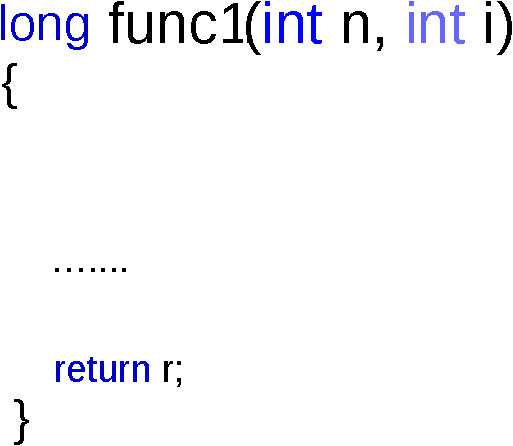
\includegraphics[width=0.35\linewidth]{figs/func_declar3.pdf}
	\end{figure}
	\begin{itemize}
		\item {You need put function implementation inside the brackets ``\{\}''}
	\end{itemize}
\end{frame}

\begin{frame}[fragile]{Define a function (4)}
\begin{itemize}
	\item {Now, let's think about how to implement fact()}
	\begin{enumerate}
		\item {For i from n to 1 do}
		\item {~~r = r*i}
		\item {~~$i--$}
		\item {End-for}
		\item {return r}
	\end{enumerate}
\end{itemize}

\end{frame}

\begin{frame}[fragile]{Define a function (4): separate declaration from definition}
\vspace{-0.2in}
\begin{columns}
\begin{column}{0.48\linewidth}
\begin{lstlisting}
long fact(int i); 
int main()
{
   int i = 5;
   long f = 0;
   f = fact(i);
   return 0; 
}
long fact(int i)
{
   long n = 1;
   if(i < 0)
     return 0;
   else if(i == 0)
     return 1;

\end{lstlisting}
\end{column}
\begin{column}{0.48\linewidth}
\begin{lstlisting}[firstnumber=16]
   else
   {
       while(i>0)
       {
          n = n*i;
          i--;
       }
   }
   return n;
}

\end{lstlisting}
\end{column}
\end{columns}
\end{frame}

\begin{frame}[fragile]{Define a function (5): combine declaration with definition}
\vspace{-0.2in}
\begin{columns}
\begin{column}{0.48\linewidth}
\begin{lstlisting}
long fact(int i)
{
   long n = 1;
   if(i < 0)
     return 0;
   else if(i == 0)
     return 1;
   else
   {
       while(i>0)
       {
          n = n*i;
          i--;
       }
   }
   return n;
}
\end{lstlisting}
\end{column}
\begin{column}{0.48\linewidth}
\begin{lstlisting}[firstnumber=18]
int main()
{
   int i = 5;
   long f = 0;
   f = fact(i);
   return 0; 
}

\end{lstlisting}
\end{column}
\end{columns}
\end{frame}

\section{Functions with Examples}
\label{sec:example}
\begin{frame}[fragile]{Example-1}
\begin{itemize}
	\item {Define a function to calculate the area of a circle}
	\item {Arguments and Parameters should be matched}
\end{itemize}
\begin{lstlisting}
float arear(float r, float pi)
{
   float a = 0;
   a = r*r*pi;
}

int main()
{
   float r = 1.5;
   const float pi = 3.1415926;
   r = area(r, pi);
   return 0;
}
\end{lstlisting}
\end{frame}

\begin{frame}[fragile]{Example-2 (1)}
\begin{itemize}
	\item {Define a function to check whether a number is Palindrome number}
	\item {such as: \textcolor{red}{321123}, \textcolor{red}{1221}, \textcolor{red}{121}}
\end{itemize}
\begin{center}
	\Large{
	Think about this in 5 minutes ...
	}
\end{center}
\end{frame}

\begin{frame}[fragile]{Example-2 (2)}
\begin{lstlisting}
int isPalindr(int n)
{
    int b = n, r = 0;
    while(b > 0){
        r = r*10+b%10;
        b = b/10;
    }
    if(n == r){
        return 1;
    }else{
        return 0;
    }
}
int main(){
   int a = 515;
   if(isPalindr(a)){
      printf("%d is Palindrome number\n", a);
   }
   return 0;
}
\end{lstlisting}
\end{frame}



\begin{frame}[fragile]{Example-3: perfect number (1)}
\begin{itemize}
	\item {1. Define a function to jugde whether an integer is a \textbf{perfect number}}
	\item {Perfect number: number equals to the sum of all its factors}
	\item {6 = 1 + 2 + 3}
	\item {2. Call it to output all the perfect numbers in range [2, 300]}
\end{itemize}
\begin{center}
	\Large{Think about this problem in 5 minutes...}
\end{center}
\end{frame}

\begin{frame}[fragile]{Example-3: perfect number (2)}
\begin{itemize}
	\item {1. Define a function to jugde whether an integer is a \textbf{perfect number}}
	\item {Perfect number: number equals to the sum of all its factors}
	\item {6 = 1 + 2 + 3}
	\item {2. Call it to output all the perfect numbers in range [2, 300]}
\end{itemize}
\begin{enumerate}
	\item {Given a number}
	\item {We should work out all its factors}
	\item {Sum all the factors up}
	\item {See whether it is equal to the number}
	\item {We should use \% operator a lot}
\end{enumerate}
\end{frame}

\begin{frame}[fragile]{Example-3: perfect number (3)}
\begin{itemize}
	\item {1. Define a function to jugde whether an integer is a \textbf{perfect number}}
	\item {\textbf{Perfect number}: number equals to the sum of all its factors}
	\item {6 = 1 + 2 + 3}
	\item {2. Call it to output all the perfect numbers in range [2, 300]}
	\item {Steps:}
	\begin{enumerate}
		\item {Give n}
		\item {~~For i from 2 to n do}
		\item {~~~~check whether n is dividable by i}
		\item {~~~~if yes, sum up}
		\item {~~Check wether sum equals to n}
		\item {~~Return \textcolor{red}{1} or \textcolor{red}{0}}
	\end{enumerate}
	\item {Let's do it now!!}
\end{itemize}
\end{frame}

\begin{frame}[fragile]{Example-3: perfect number (4)}
\vspace{-0.15in}
\begin{columns}
\begin{column}{0.55\linewidth}
\begin{enumerate}
	\item {Give n}
	\item {~~For i from 2 to n do}
	\item {~~~~check whether n is dividable by i}
	\item {~~~~if yes, sum up}
	\item {~~Check wether sum equals to n}
	\item {~~Return \textcolor{red}{1} or \textcolor{red}{0}}
\end{enumerate}
\end{column}
\begin{column}{0.45\linewidth}
\begin{lstlisting}
int isPerfect(int n)
{
    int i = 0, sum = 1;
    int up = ceil(n/2.0);
    for(i = 2; i < up; i++)
    {
        if(n%i == 0)
        {
           sum += i;
        }
    }
    if(sum == n)
      return 1;
    else 
      return 0;
}
\end{lstlisting}
\end{column}
\end{columns}
\end{frame}

\begin{frame}[fragile]{Example-3: perfect number (5)}
\vspace{-0.16in}
\begin{columns}
\begin{column}{0.48\linewidth}
\begin{lstlisting}[linewidth=0.95\linewidth]
#include <stdio.h>
#include <math.h>
int isPerfect(int n)
{
    int i = 0, sum = 1;
    int up = ceil(sqrt(n));
    for(i = 2; i < up; i++)
    {
        if(n%i == 0)
        {
           sum += i;
        }
    }
    if(sum == n)
      return 1;
    else 
      return 0;
}
\end{lstlisting}
\end{column}
\begin{column}{0.48\linewidth}
\begin{lstlisting}[firstnumber=19, linewidth=0.95\linewidth]
int main()
{
   int i = 0;
   for(i = 2; i <= 300; i++)
   {
      if(isPerfect(i))
      {
         printf("%d\n", i);
      }
   }
   return 0;
}
\end{lstlisting}
\end{column}
\end{columns}
\end{frame}



\begin{frame}[fragile]{Example-4: Armstrong number (1)}
\vspace{-0.16in}
\begin{itemize}
	\item {Define a function to check whether a number is Amstrong number}
	\item {For one digits: $1^1$ = 1}
	\item {For three digits: $1^3$ + $5^3$+$3^3$ = 153}
	\item {For four digits: $1^4 + 6^4 + 3^4 + 4^4$ = 1634}
\end{itemize}
\begin{center}
	\Large{
	   Think about this in 5 minutes ...
	}
\end{center}
\end{frame}

\begin{frame}[fragile]{Example-4: Armstrong number (2)}
\vspace{-0.16in}
\begin{columns}
\begin{column}{0.48\linewidth}
\begin{lstlisting}[linewidth=0.95\linewidth]
#include <stdio.h>
int isArms(int n)
{
  int nd = 0, s = 0, b = 0;
  int a = n, i = 0, t = 0;
  while(a > 0){
     a = a/10;
     nd++;
  }
  a = n;
  while(a > 0){
    b = a%10;
    t = 1;
    for(i = 0; i < nd; i++){
       t = t*b;
    }
    s += t;
    a  = a/10;
  }//end-while(a)
\end{lstlisting}
\end{column}
\begin{column}{0.48\linewidth}
\begin{lstlisting}[firstnumber=20, linewidth=0.95\linewidth]
   if(s == n)
     return 1;
   else
     return 0;
}

int main()
{
 int i = 1;
 for(i=1; i<100000; i++)
 {
     if(isArms(i) == 1)
     {
        printf("%6d ", i);
     }
 }
 return 0;
}
\end{lstlisting}
\end{column}
\end{columns}
\end{frame}


\begin{frame}[fragile]{Function definition: a summary}
\LARGE{
\begin{itemize}
	\item {Princeples in function definition}
	\begin{enumerate}
		\item {Remember return type, if there is no need, put \textcolor{blue}{void}}
		\item {Give a unique and self-telling name to your function}
		\item {Define function first, then you can call it (just as variable in C)}
		\item {Parameters along with the type appear in pair}
		\item {Parameters are transferred by \textcolor{red}{value}}
	\end{enumerate}
\end{itemize}
}
\end{frame}

\begin{frame}[fragile]{Parameter Transfer (1)}
\begin{figure}
	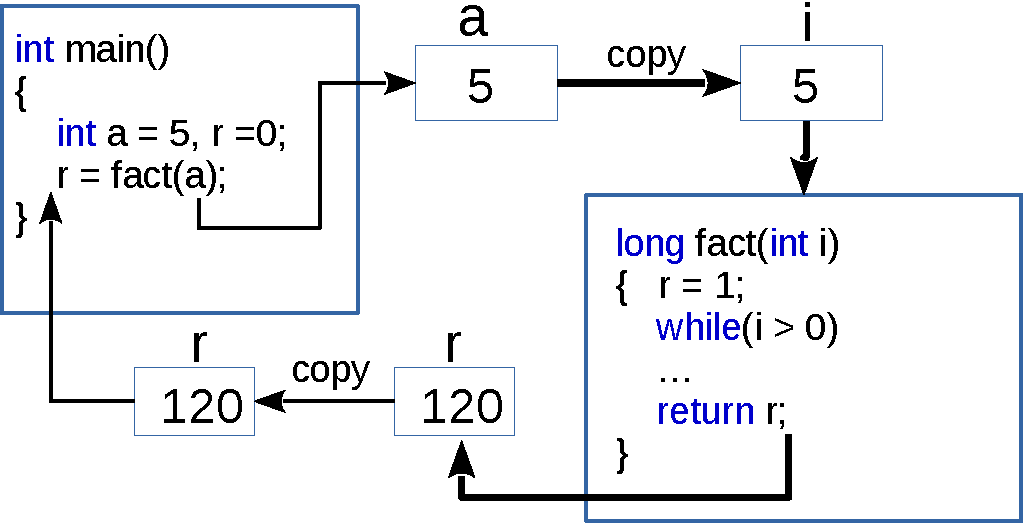
\includegraphics[width=0.85\linewidth]{figs/arg2para.pdf}
\end{figure}
\begin{itemize}
	\item {Parameters are transferred in \textcolor{red}{by value} not \textbf{by address}}
\end{itemize}
\end{frame}

\begin{frame}[fragile]{Parameter Transfer (2)}
\begin{itemize}
	\item {Let's consider a simple coding problem}
	\item {Given integers \textit{a} and \textit{b}}
	\item {You are required to swap their values}
	\item {For example, a = 5, b = 8}
	\item {After swapping, it becomes a = 8, b = 5}
\end{itemize}

\end{frame}

\begin{frame}[fragile]{Parameter Transfer (3)}
\begin{itemize}
	\item {You are required to swap their values}
	\item {For example, a = 5, b = 8}
	\item {After swapping, it becomes a = 8, b = 5}
\end{itemize}
\begin{lstlisting}
int main()
{
    int a = 5, b = 8;
    int tmp;
    printf("a = %d, b = %d\n", a, b);
    tmp = a; a = b;
    b = tmp;
    printf("a = %d, b = %d\n", a, b);
    return 0;
}
\end{lstlisting}

\end{frame}

\begin{frame}[fragile]{Parameter Transfer (4)}
\begin{itemize}
	\item {Now, let's do it by a function}
\end{itemize}
\begin{lstlisting}
#include <stdio.h>
void swap(int a, int b)
{
   int tmp = a;
   a = b; b = tmp;
   return ;
}
int main()
{
    int a = 5, b = 8;
    printf("a = %d, b = %d\n", a, b);
    swap(a, b);
    printf("a = %d, b = %d\n", a, b);
}
\end{lstlisting}
\end{frame}

\begin{frame}[fragile]{Parameter Transfer (5)}
\begin{itemize}
	\item {The result is against our will, why???}
\end{itemize}
\begin{columns}
\begin{column}{0.65\linewidth}
\begin{lstlisting}
#include <stdio.h>
void swap(int a, int b)
{
   int tmp = a;
   a = b; b = tmp;
   return ;
}
int main()
{
    int a = 5, b = 8;
    printf("a = %d, b = %d\n", a, b);
    swap(a, b);
    printf("a = %d, b = %d\n", a, b);
    return 0;
}
\end{lstlisting}
\end{column}
\begin{column}{0.3\linewidth}
[Output:]
\begin{lstlisting}
a = 5, b = 8
a = 5, b = 8
\end{lstlisting}
\end{column}
\end{columns}
\end{frame}

\begin{frame}[fragile]{Parameter Transfer (6)}
\begin{figure}
	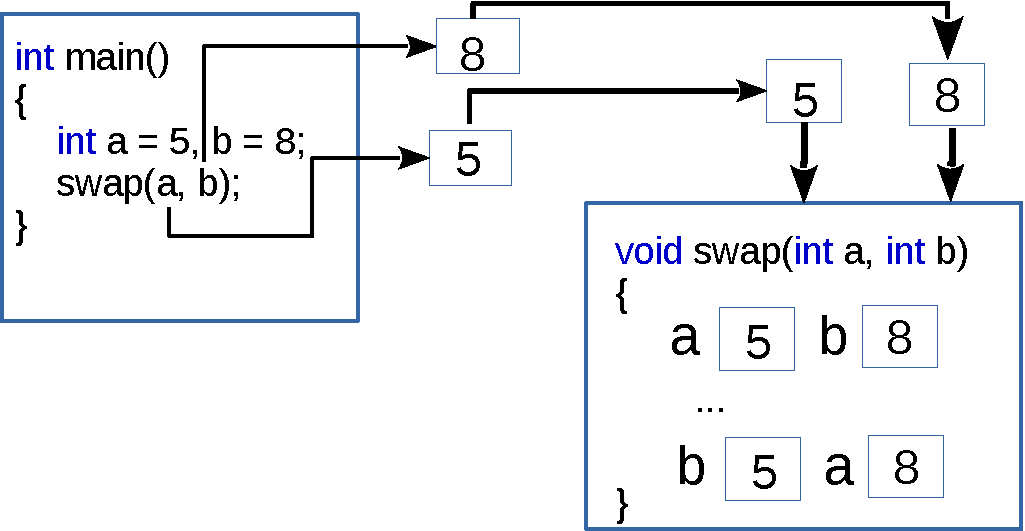
\includegraphics[width=0.85\linewidth]{figs/swap.pdf}
\end{figure}
\begin{itemize}
	\item {Parameters are transferred in \textcolor{red}{by value} not \textbf{by address}}
\end{itemize}
\end{frame}

\begin{frame}[fragile]{Function Calling again (1)}
\begin{figure}
	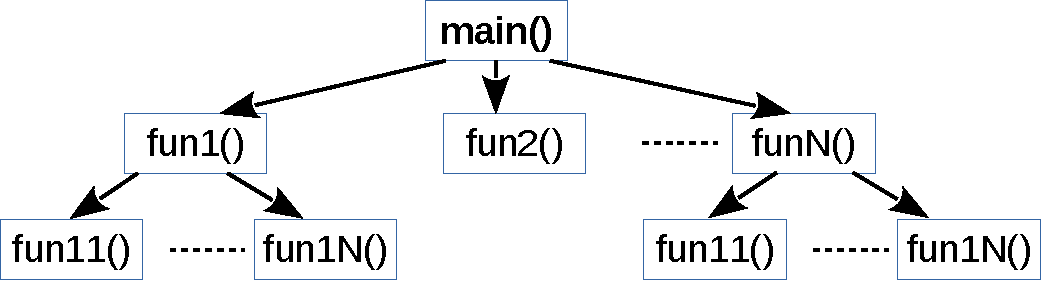
\includegraphics[width=0.8\linewidth]{figs/func_call.pdf}
\end{figure}
\begin{itemize}
	\item {Function can be called in a cascaded manner}
	\item {`main' cannot be called}
	\item {Functions are not necessarily called by `main' directly}
\end{itemize}
\end{frame}

\begin{frame}[fragile]{Function Calling again (2)}
\begin{itemize}
	\item {Parameters are transferred in \textcolor{red}{by value} not \textbf{by address}}
	\item {Arguments and Parameters should be matched}
\end{itemize}
\begin{lstlisting}
float calc(int n, float a, short int c)
{
    return (a*a*n+c);
}
int main()
{
   int n = 2;
   short int w = 4;
   float x = 4.12, r = 0;
   r = 3*calc(n, x, w);
   return 0;
}
\end{lstlisting}
\end{frame}
\section{Recursive Functions}
\label{sec:recurs}
\begin{frame}<beamer>
    \frametitle{Outline}
    \tableofcontents[currentsection]
\end{frame}

\begin{frame}[fragile]{Recursive Function (1)}
\begin{itemize}
	\item {We already know that function is allowed to call any other function}
	\item {Function is allowed to call itself, this is called \textbf{recursive}}
	\item {It looks like following}
\end{itemize}
\begin{lstlisting}
int func2(int n);
int func1(int n)
{
   int a = 2*func1(n-2);
   ...
   int b = func2(n-3);
   return (a+b);
}
\end{lstlisting}

\begin{itemize}
	\item {Noticed that ``func1'' has been called inside ``func1''}
	\item {The scale of the problem decreases in each calling}
\end{itemize}

\end{frame}

\begin{frame}[fragile]{Recursive Function: how it works (1)}
\vspace{-0.08in}
\begin{columns}
\begin{column}{0.48\linewidth}
\begin{lstlisting}
long fact(int n)
{
   long a = 0;
   if (n < 0)
     a = 0;
   else if(n == 1 || n == 0)
    a  = 1;
   else
    a = n*fact(n-1);
    
   return a;
}
\end{lstlisting}
\end{column}
\begin{column}{0.45\linewidth}
\begin{lstlisting}
long fact(int n)
{
   long a = 1;
   int i = 0;
   if(n < 0)
     return 0;
   for(i = n; i > 0; i--)
   {
      a = a*i;
   }
   return a;
}
\end{lstlisting}
\end{column}
\end{columns}
\vspace{-0.16in}
\begin{lstlisting}
int main()
{
   int n = 4, b = 0;
   b = fact(n);
   printf("fact(%d) = %d\n", n, b);
   return 0;
}
\end{lstlisting}
\end{frame}

\begin{frame}[fragile]{Recursive Function: how it works (2)}
\vspace{0.1in}
\begin{itemize}
	\item {``fact'' calls itself until the \textbf{bottom} is reached}
	\item {Noticed that the scale of the problem decreases gradually}
	\item {Advantage: simple}
	\item {Darkside: requires a lot of memory}
\end{itemize}
\vspace{0.2in}
\begin{figure}
	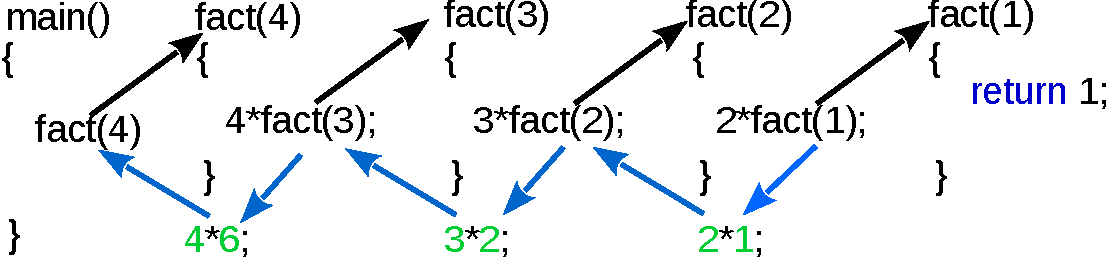
\includegraphics[width=0.95\linewidth]{figs/recurs.pdf}
\end{figure}
\begin{itemize}
	\item {Suggesion: try to avoid to use recursive function}
\end{itemize}
\end{frame}

\begin{frame}{Recursive Function: Hanoi Tower Problem}
\begin{itemize}
	\item {One is allowed to move one disc from one beam to another a day}
	\item {Move all 64 discs from beam A to C}
\end{itemize}
%\vspace{0.2in}
\begin{figure}
	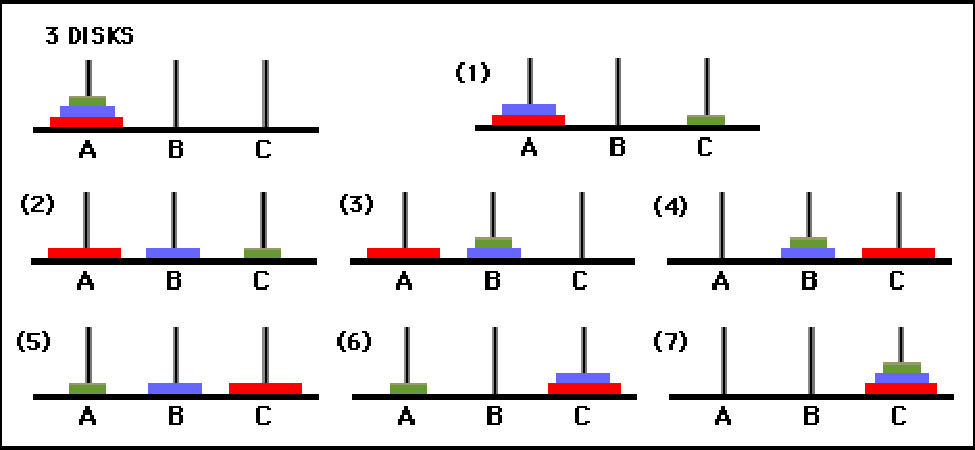
\includegraphics[width=0.85\linewidth]{figs/hanoi.pdf}
\end{figure}
\begin{itemize}
	\item {\textbf{It would not be fulfilled even till the end of this world!!}}
\end{itemize}
\end{frame}

\begin{frame}[fragile]{Source code for Hanoi Tower (1)}
\vspace{-0.15in}
\begin{lstlisting}[xleftmargin=0.02\linewidth, linewidth=0.85\linewidth]
#include <stdio.h>
void hanoi(int n, char b1, char b2, char b3)
{
    if(n == 1)
    {
        printf("%c ----> %c \n", b1, b3);
    }else if(n == 2)
    {
        printf("%c ----> %c\n", b1, b2);
        printf("%c ----> %c\n", b1, b3);
        printf("%c ----> %c\n", b2, b3);
    }else{
        hanoi(n-1, b1, b3, b2);
        printf("%c ----> %c\n", b1, b3);
        hanoi(n-1, b2, b1, b3);
    }
}
\end{lstlisting}
\vspace{-0.1in}

\end{frame}

\begin{frame}[fragile]{Source code for Hanoi Tower (2)}
\vspace{-0.15in}
\begin{lstlisting}[firstnumber=19, xleftmargin=0.02\linewidth, linewidth=0.85\linewidth]
int main()
{
   int n = 20;
   printf("Input n: ");
   scanf("%d", &n);
   hanoi(n, 'A', 'B', 'C');
}
\end{lstlisting}
\begin{enumerate}
	\item {Move top \textbf{n-1} plates from \textcolor{red}{\textbf{A}} to \textcolor{red}{\textbf{B}} via \textcolor{red}{\textbf{C}}}
	\item {Move the \textbf{bottom one} to \textcolor{red}{\textbf{C}}}
	\item {Move \textbf{n-1} plates from \textcolor{red}{\textbf{B}} to \textcolor{red}{\textbf{C}} via \textcolor{red}{\textbf{A}}}
\end{enumerate}
\end{frame}
\section{Visibility and Life-cycle of Variables}
\label{sec:vars}
\begin{frame}<beamer>
    \frametitle{Outline}
    \tableofcontents[currentsection]
\end{frame}

\begin{frame}[fragile]{Visibility and Life-cycle of Variables (1)}
\begin{itemize}
	\item {We take something for granted before}
	\item {Now we study them in detail}
	\begin{enumerate}
		\item {Could we use the same variable name in different functions?}
		\item {Could we use the same variable name in the same functions?}
		\item {Could different functions share the same variable?}
		\item {When a variable is born, when it dies??}
	\end{enumerate}
\end{itemize}

\end{frame}

\begin{frame}[fragile]{Visibility and Life-cycle of Variables (2)}
\begin{enumerate}
	\item {Could we use the same variable name in different functions?}
\end{enumerate}
\begin{columns}
\begin{column}{0.53\linewidth}
\begin{lstlisting}[linewidth=0.9\linewidth, xleftmargin=0.05\linewidth]
int func1(int n)
{
   int r = 3, a = 1;
   return (r*n+a);
}
float func2(int n, float a)
{
   float r = 1;
   int i = 0;
   for(i = 0; i < n; i++)
   {
      r = r*a;
   }
   return r;
}
\end{lstlisting}
\end{column}
\begin{column}{0.46\linewidth}
\begin{itemize}
	\item {The answer is \textcolor{red}{Yes}}
	\item {The visibility is inside function only}
	\item {It is born when the function is called}
	\item {It dies when calling is done}
\end{itemize}
\end{column}
\end{columns}
\end{frame}

\begin{frame}[fragile]{Visibility and Life-cycle of Variables (3)}
\begin{enumerate}
	\setcounter{enumi}{1}
	\item {Could we use the same variable name in the same function?}
\end{enumerate}
\begin{columns}
\begin{column}{0.55\linewidth}
\begin{lstlisting}[linewidth=0.9\linewidth, xleftmargin=0.05\linewidth]
float func2(int n, float a)
{
  float r = 1;
  int r = 0;
  int i = 0;
  float i = 0;
  for(i = 0; i < n; i++, r++)
  {
     r = r*a;
  }
  return r;
}
\end{lstlisting}
\end{column}
\begin{column}{0.44\linewidth}
\begin{itemize}
	\item {The answer is \textcolor{red}{No}}
	\item {Codes on the left cannot pass the compilation}
	\item {Basically, it is ambiguous}
	\item {Imagine there are two \textbf{Li Min}s in your class}
\end{itemize}
\end{column}
\end{columns}
\end{frame}

\begin{frame}[fragile]{Visibility and Life-cycle of Variables (4-1)}
\begin{enumerate}
	\setcounter{enumi}{2}
	\item{Could different functions share the same variable?}
\end{enumerate}
\begin{columns}
\begin{column}{0.52\linewidth}
\begin{lstlisting}[xleftmargin=0.05\linewidth, linewidth=0.85\linewidth]
int x, y;
void swap()
{
  int t;
  t = x; x = y; y = t;
  return ;
}
int main()
{
   x = 3, y = 5;
   swap();
   printf("x = %d\n", x);
   printf("y = %d\n", y);
   return 0;
}
\end{lstlisting}
\end{column}
\begin{column}{0.47\linewidth}
\begin{itemize}
	\item {The answer is \textcolor{red}{Yes}}
	\item {They are called global variables}
	\item {They are visible to all functions in this \textbf{file}}
	\item {They are defined outside of functions}
	\item {They are born when ``main'' is called}
	\item {They die when calling of ``main'' complete}
\end{itemize}
\end{column}
\end{columns}
\end{frame}

\begin{frame}[fragile]{Visibility and Life-cycle of Variables (4-2)}
\begin{enumerate}
	\setcounter{enumi}{2}
	\item{Could different functions share the same variable?}
\end{enumerate}
\vspace{-0.15in}
\begin{columns}
\begin{column}{0.44\linewidth}
\begin{lstlisting}[xleftmargin=0.05\linewidth]
#include <stdio.h>
int x, y;
void swap()
{
  int t;
  t = x; x = y; y = t;
  return ;
}
int main()
{
   x = 3, y = 5;
   swap();
   printf("x = %d\n", x);
   printf("y = %d\n", y);
   return 0;
}
\end{lstlisting}
\end{column}
\begin{column}{0.54\linewidth}
\begin{lstlisting}[linewidth=0.98\linewidth]
#include <stdio.h>
void swap(int a, int b)
{
   int tmp = a;
   a = b; b = tmp;
   return ;
}
int main()
{
  int a = 5, b = 8;
  swap(a, b);
  printf("a = %d, b = %d", a,b);
  return 0;
}
\end{lstlisting}
\end{column}
\end{columns}
\end{frame}

\begin{frame}[fragile]{Visibility and Life-cycle of Variables (5)}
\begin{enumerate}
	\setcounter{enumi}{4}
		\item {When a variable is born, when it dies??}
\end{enumerate}
\begin{columns}
\begin{column}{0.55\linewidth}
\begin{lstlisting}[linewidth=0.9\linewidth, xleftmargin=0.02\linewidth]
int incr(int a)
{
  static int x = 3;
  x = x + a;
  //printf("x = %d\n", x);
  return x;
}
int main()
{
   int i = 0, a = 0;
   for(i = 0; i < 4; i++)
   {
       a = incr(i);
       printf("a = %d\n", a); 
   }
   return 0;
}
\end{lstlisting}
\end{column}
\begin{column}{0.44\linewidth}
\begin{itemize}
	\item {When you put ``\textbf{static}'' before a local variable}
	\item {Its life-cycle becomes as long as global variable}
	\item {It is born when ``main'' is called}
	\item {It dies when calling of ``main'' complete}
	\item {However, it is only visible \underline{within the function}}
\end{itemize}
\end{column}
\end{columns}
\end{frame}

\begin{frame}[fragile]{Visibility and Life-cycle of Variables (6)}
\vspace{0.1in}
\begin{figure}
	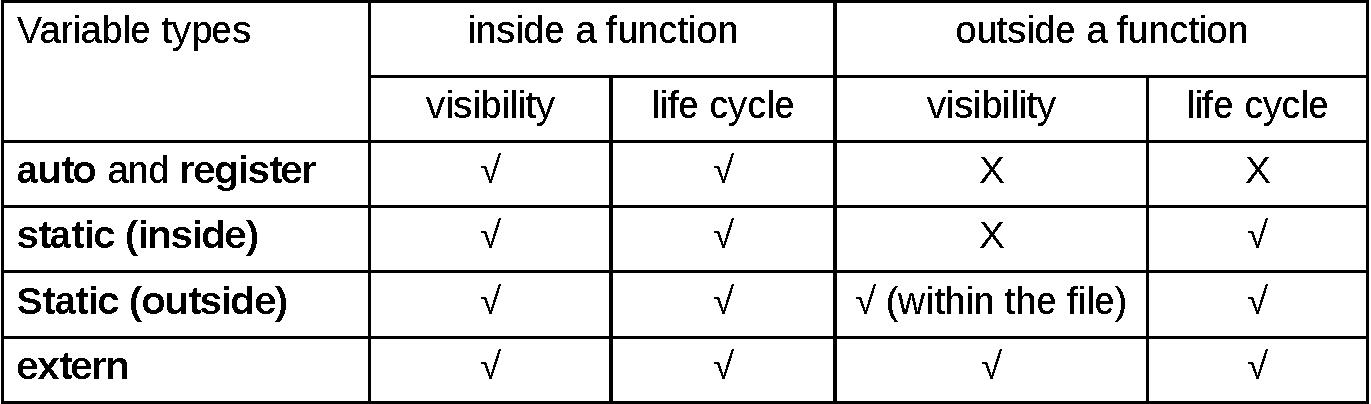
\includegraphics[width=0.8\linewidth]{figs/extern_var_eng.pdf}
\end{figure}
\begin{itemize}
	\item {It is NOT recommended to use global variables}
	\item {Advantage: you can transfer value easily}
	\item {Darkside}
	\begin{itemize}
		\item {You do NOT know where they have been changed}
		\item {Hard to debug your code}
		\item {Your code will be very messy!!!}
	\end{itemize}
\end{itemize}
\end{frame}
\section{Precompilation Instructions and Macros}
\label{sec:macro}
\begin{frame}<beamer>
    \frametitle{Outline}
    \tableofcontents[currentsection]
\end{frame}
\begin{frame}{Precompilation: the Concept (1)}
\begin{itemize}
	\item {It happens before we compile codes to binary}
	\item {Preprocess the codes}
	\item {There are instrustions we use to communicate with the compiler}
\end{itemize}

\begin{figure}
	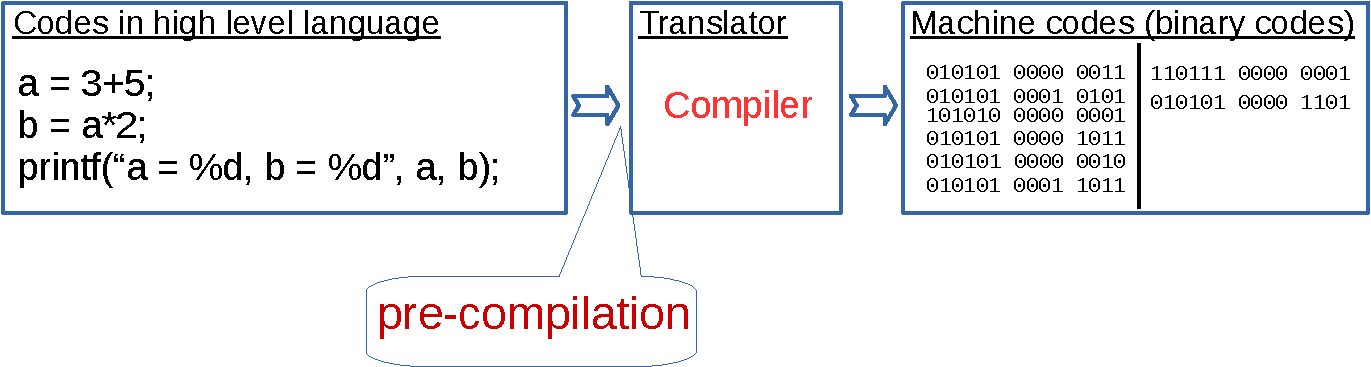
\includegraphics[width=0.9\linewidth]{figs/compil1.pdf}
\end{figure}

\begin{itemize}
	\item {They are executed before compilation is undertaken}
\end{itemize}

\end{frame}

\begin{frame}{Precompilation: the Concept (2)}
\begin{figure}
	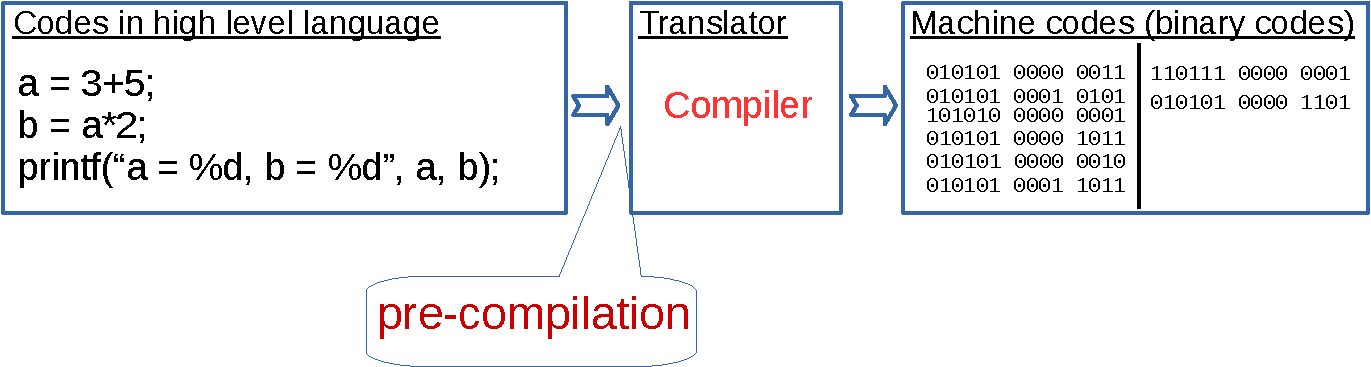
\includegraphics[width=0.9\linewidth]{figs/compil1.pdf}
\end{figure}

\begin{itemize}
	\item {There are instrustions we use to communicate with the compiler}
	\item {They all start with ``\textcolor{red}{\#}'', pronounced as ``sharp''}
	\begin{enumerate}
		\item {\#\textcolor{blue}{include} header file or full path of file}
		\item {\#\textcolor{blue}{define} MACRO}
		\item {\#\textcolor{blue}{if}...\#\textcolor{blue}{else} or \#\textcolor{blue}{if}...\#\textcolor{blue}{else if} MACRO}
		\item {\#\textcolor{blue}{ifndef} MACRO}
		\item {\#\textcolor{blue}{endif}}
	\end{enumerate}
\end{itemize}

\end{frame}

\begin{frame}[fragile]{Precompilation instruction: \#\textcolor{blue}{include} (1)}
\begin{itemize}
	\item {It tells the compiler following thing}
	\begin{enumerate}
		\item {A header file is required to compile the code}
		\item {In the header file, the function that is called in the code is declared}
		\item {Where the compiler is able to find the file}
	\end{enumerate}
\end{itemize}
\begin{columns}
\begin{column}{0.45\linewidth}
\begin{lstlisting}
#include <stdio.h>

\end{lstlisting}
\end{column}
\begin{column}{0.45\linewidth}
\begin{lstlisting}
#include "myfunc.h"

\end{lstlisting}
\end{column}
\end{columns}
\begin{itemize}
	\item {$<$stdio.h$>$ tells the compiler to search in the system default path}
	\item {"myfunc.h" tells the compiler to \textcolor{red}{1}. search in the directed path, \textcolor{red}{2}. then go to system default path}
\end{itemize}
\end{frame}

\begin{frame}[fragile]{Precompilation instruction: \#\textcolor{blue}{include} (2)}
\begin{columns}
\begin{column}{0.52\linewidth}
[myfunc.h]
\begin{lstlisting}[linewidth=0.95\linewidth]
float mypow(float base, int n)
{
   float r = 1;
   int i = 0;
   
   if(n == 0)
   rerturn r;
   
   for(i = 1; i <= n; i++)
   {
      r = base*r;
   }
   return r;
}
\end{lstlisting}
\end{column}
\begin{column}{0.46\linewidth}
[main.c]
\begin{lstlisting}
#include "myfunc.h"
#include <stdio.h>
int main()
{
  float r = mypow(3.14, 3);
  printf("r = %f\n", r);
  return 0;
}
\end{lstlisting}
\end{column}
\end{columns}
\end{frame}

\begin{frame}[fragile]{Instruction for Macros: \#\textcolor{blue}{define} (1)}
\begin{itemize}
	\item {\#\textcolor{blue}{define} allows user to define constants or functions}
	\item {These constants and functions can be later called in the code}
	\item {As a convention, we CAPITALIZE everything}
	\item {However, it is possible that PI is defined elsewhere}
\end{itemize}

\begin{columns}
\begin{column}{0.44\linewidth}
\begin{lstlisting}[xleftmargin=0.02\linewidth]
#define PI 3.1415926
#include <stdio.h>
int main()
{
  float a = 0, r = 4.5;
  a = PI*r*r;
  printf("a = %f\n", a);
  return 0;
}
\end{lstlisting}
\end{column}
\begin{column}{0.14\linewidth}
\begin{center}
\vspace{0.6in}
$\Longrightarrow$
\end{center}
\end{column}
\begin{column}{0.41\linewidth}
\begin{block}{After pre-compilation}
\end{block}
\begin{lstlisting}
#define PI 3.1415926
#include <stdio.h>
int main()
{
  float a = 0, r = 4.5;
  a = 3.1415926*r*r;
  printf("a = %f\n", a);
  return 0;
}
\end{lstlisting}
\end{column}
\end{columns}
\end{frame}

\begin{frame}[fragile]{Instruction for Macros: \#\textcolor{blue}{define} (2)}
\begin{itemize}
	\item {However, it is possible that PI is defined elsewhere}
\end{itemize}

\begin{columns}
\begin{column}{0.44\linewidth}
\begin{lstlisting}
#define PI 3.1415926
#include <stdio.h>
int main()
{
  float a = 0, r = 4.5;
  a = PI*r*r;
  printf("a = %f\n", a);
  return 0;
}
\end{lstlisting}
\end{column}
\begin{column}{0.44\linewidth}
\begin{lstlisting}
#ifndef PI
#define PI 3.1415926
#endif
#include <stdio.h>
int main()
{
  float a = 0, r = 4.5;
  a = PI*r*r;
  printf("a = %f\n", a);
  return 0;
}
\end{lstlisting}
\end{column}
\end{columns}
\end{frame}

\begin{frame}[fragile]{Instruction for Macros: \#\textcolor{blue}{define} (3)}
\begin{itemize}
	\item {Pay attention that the constant has NO type}
	\item {We can similarly define Macro function}
\end{itemize}
\begin{columns}
\begin{column}{0.40\linewidth}
\begin{lstlisting}
#define MULT(x,y) x*y+y
#include <stdio.h>
int main()
{
  float a = 2, r = 4.5;
  a = MULT(a, r);
  printf("a = %f\n", a);
  return 0;
}
\end{lstlisting}
\end{column}
\begin{column}{0.40\linewidth}
\begin{lstlisting}
#ifndef MULT
#define MULT(x,y) x*y+y
#endif
#include <stdio.h>
int main()
{
  float a = 2, r = 4.5;
  a = MULT(a, r)*4;
  printf("a = %f\n", a);
  return 0;
}
\end{lstlisting}
\end{column}
\end{columns}
\begin{itemize}
	\item {Please work out the output for each ...}
\end{itemize}
\end{frame}

\begin{frame}[fragile]{Instruction for Macros: \#\textcolor{blue}{define} (4)}
\begin{itemize}
	\item {Pay attention that the constant has NO type}
	\item {We can similarly define Macro function}
\end{itemize}
\begin{columns}
\begin{column}{0.44\linewidth}
\begin{lstlisting}[linewidth=0.9\linewidth]
#ifndef MULT
#define MULT(x,y) x*y+y
#endif
#include <stdio.h>
int main()
{
  float a = 2, r = 4.5;
  a = MULT(a, r)*4;
  printf("a = %f\n", a);
  return 0;
}
\end{lstlisting}
\end{column}
\begin{column}{0.1\linewidth}
\begin{center}
\vspace{0.6in}
$\Longrightarrow$
\end{center}
\end{column}
\begin{column}{0.40\linewidth}
\begin{block}{After pre-compilation}
\end{block} 
\begin{lstlisting}
#include <stdio.h>
int main()
{
  float a = 2, r = 4.5;
  a = a*r+r*4;
  printf("a = %f\n", a);
  return 0;
}
\end{lstlisting}
\end{column}
\end{columns}
\begin{itemize}
	\item {It is better to put the bracket on the whole}
\end{itemize}
\end{frame}

\begin{frame}[fragile]{Instruction for Macros: \#\textcolor{blue}{define} (5)}
\begin{itemize}
	\item {Pay attention that the constant has NO type}
	\item {We can similarly define Macro function}
\end{itemize}
\begin{columns}
\begin{column}{0.44\linewidth}
\begin{lstlisting}[xleftmargin=0.05\linewidth]
#ifndef MULT
#define MULT(x,y) (x*y+y)
#endif
#include <stdio.h>
int main()
{
  float a = 2, r = 4.5;
  a = MULT(a, r)*4;
  printf("a = %f\n", a);
  return 0;
}
\end{lstlisting}
\end{column}
\begin{column}{0.14\linewidth}
\begin{center}
\vspace{0.6in}
$\Longrightarrow$
\end{center}
\end{column}
\begin{column}{0.42\linewidth}
\begin{block}{After pre-compilation}
\end{block} 
\begin{lstlisting}
#include <stdio.h>
int main()
{
  float a = 2, r = 4.5;
  a = (a*r+r)*4;
  printf("a = %f\n", a);
  return 0;
}
\end{lstlisting}
\end{column}
\end{columns}
\begin{itemize}
	\item {It is better to put the bracket on the whole}
\end{itemize}
\end{frame}

\begin{frame}[fragile]{Instruction for Macros: \#\textcolor{blue}{define} (6)}
\begin{itemize}
	\item {It is literally replacement all the time}
\end{itemize}
\begin{columns}
\begin{column}{0.42\linewidth}
\begin{lstlisting}
#ifndef HI
#define HI "hello"
#define WD	world
#endif
#include <stdio.h>
int main()
{
  printf("HI");
  printf("\n");
  printf(WD);
  printf("\n");
  printf(HI);
  return 0;
}
\end{lstlisting}
\end{column}
\begin{column}{0.40\linewidth}
[Output]
\begin{lstlisting}
??
??
\end{lstlisting}
\end{column}
\end{columns}
\end{frame}

\begin{frame}[fragile]{Instruction for Macros: \#\textcolor{blue}{define} (7)}
\begin{itemize}
	\item {It is literally replacement all the time}
\end{itemize}
\begin{columns}
\begin{column}{0.46\linewidth}
\begin{lstlisting}
#ifndef HI
#define HI "hello"
#define WD	world
#endif
#include <stdio.h>
int main()
{
  printf("HI");
  printf("\n");
  //printf(WD); //<--mistake
  printf("\n");
  printf(HI);
  return 0;
}
\end{lstlisting}
\end{column}
\begin{column}{0.35\linewidth}

[after comment out \textcolor{blue}{line 10},\\output]
\begin{lstlisting}
HI
hello
\end{lstlisting}
\end{column}
\end{columns}
\end{frame}

\begin{frame}[fragile]{Instruction for Macros: \#\textcolor{blue}{ifdef} (1)}
\begin{itemize}
	\item {We can use Macro to control the compilation}
\end{itemize}
\vspace{-0.2in}
\begin{columns}
\begin{column}{0.48\linewidth}
\begin{lstlisting}
#define DEBUG
#include <stdio.h>
int main()
{
  int i = 0, j = 1;
  for(i = 0; i < 5; i++)
  {
     j = i*2+1;
     #ifdef DEBUG
       printf("j = %f\n", j);
     #endif
  }
  return 0;
}
\end{lstlisting}
\end{column}
\begin{column}{0.48\linewidth}
\begin{lstlisting}
//#define DEBUG
#include <stdio.h>
int main()
{
  int i = 0, j = 1;
  for(i = 0; i < 5; i++)
  {
     j = i*2+1;
     #ifdef DEBUG
       printf("j = %f\n", j);
     #endif
  }
  return 0;
}
\end{lstlisting}
\end{column}
\end{columns}
\vspace{-0.2in}
\begin{itemize}
	\item {The code is compiled inside \#\textcolor{blue}{ifdef} only when ``\textbf{DEBUG}'' is defined}
\end{itemize}
\end{frame}

\begin{frame}[fragile]{Instruction for Macros: \#\textcolor{blue}{ifdef} (2)}
\begin{itemize}
	\item {Codes after pre-compilation}
\end{itemize}
\vspace{-0.2in}
\begin{columns}
\begin{column}{0.52\linewidth}
\begin{lstlisting}[xleftmargin=0.02\linewidth, linewidth=0.9\linewidth]
#define DEBUG
#include <stdio.h>
int main()
{
  int i = 0, j = 1;
  for(i = 0; i < 5; i++)
  {
     j = i*2+1;
     printf("j = %f\n", j);
  }
  return 0;
}
\end{lstlisting}
\end{column}
\begin{column}{0.47\linewidth}
\begin{lstlisting}
//#define DEBUG
#include <stdio.h>
int main()
{
  int i = 0, j = 1;
  for(i = 0; i < 5; i++)
  {
     j = i*2+1;
  }
  return 0;
}
\end{lstlisting}
\end{column}
\end{columns}
\vspace{-0.2in}
\begin{itemize}
	\item {The code is compiled inside \#\textcolor{blue}{ifdef} only when ``\textbf{DEBUG}'' is defined}
\end{itemize}
\end{frame}
\section{}
\end{document}
